\documentclass{spiral-kurs}
\def\title{Krokodyle}
\def\id{kro}
\def\TL{1~s}
\def\ML{256~MB}
\begin{document}
\makeheader
%
  Faraon złapał na gorącym uczynku złodzieja Pteppica -- rozbójnika o dobrym sercu, choć nie nazbyt porażającej inteligencji.
  Ponieważ prawo stanowi, że każdemu skazańcowi należy dać szansę przeżycia, Pteppic zostanie poddany próbie: 
  oto musi pokonać ogród-tor przeszkód faraona, pozostając żywym.
  
  Każda przeszkoda to polanka z prostokątną siatką ścieżek, podzielona ścieżkami na $a \times b$ kwadratowych pól.
  Na polach znajdują się sadzawki, w których pływają święte krokodyle -- w tej chwili główne zmartwienie Pteppica:
  
  \begin{center}
   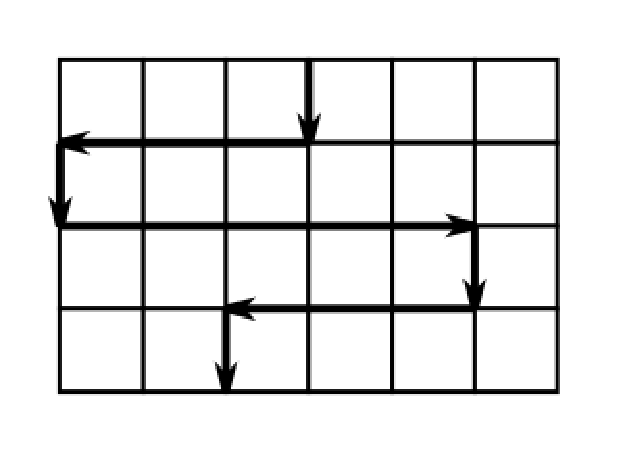
\includegraphics[width=0.3\textwidth]{grid.eps}
  \end{center}
  
  Skazaniec musi przejść od jednego do drugiego końca polanki (czyli od górnej do dolnej krawędzi siatki na rysunku). 
  Musi (z oczywistych względów) iść wzdłuż ścieżek, może na skrzyżowaniach skręcać w lewo lub w prawo, nie wolno mu się jednak cofać (czyli na rysunku: iść do góry).
  
  Dla każdej przeszkody oblicz, na ile sposobów Pteppic może ją pokonać. Ponieważ mogą to być duże liczby, wystarczy że podasz ich resztę z dzielenia przez $10000$
  (na przykład zamiast $131072$ wypisz $1072$, a zamiast $10023$ -- $23$).
  
  \section{Wejście}
  W pierwszym wierszu wejścia znajduje się liczba przeszkód $P \leq 10\,000$. W kolejnych $P$ wierszach podane są opisy przeszkód:
  każdy taki opis to dwie liczby $a$ i $b$, oznaczające odpowiednio jej szerokość oraz wysokość. Obie liczby są dodatnie, $a \leq 10,000$, $b \leq 10^9$.
  
  \section{Wyjście}
  Wypisz, dla każdej przeszkody w osobnym wierszu, liczbę sposobów, na jaką można pokonać tę przeszkodę.
                                  
    \example{0}


  \end{document}
